\chapter[IA Souveraine \& Avatar 3D]{Réalisation : Intelligence Artificielle Souveraine \& Avatar 3D}
\label{chap:ia}

\section{Architecture du LLM Souverain Qwen2.5-Coder:7b}
L'un des défis majeurs pour les infrastructures d'État consiste à bénéficier des capacités de pointe de l'IA générative sans compromettre la souveraineté des données.

\subsection{Spécifications du Modèle \& Runtime Ollama}
CyberScore TN intègre le modèle de fondation \textbf{\texttt{Qwen2.5-Coder:7b}} (format quantifié GGUF Q4\_K\_M, empreinte mémoire de 4.7 Go), exécuté localement via le runtime Ollama sur le port \texttt{25000} (avec fallback sur le port par défaut \texttt{11434}) :
\begin{itemize}
    \item \textbf{Performance de Génération de Code} : Score de 88.4\% au benchmark HumanEval, surpassant la majorité des modèles de sa catégorie et rivalisant avec GPT-4o sur la production de configurations de sécurité (fichiers \texttt{nginx.conf}, directives Apache, règles \texttt{nftables}, scripts Bash de durcissement).
    \item \textbf{Souveraineté Intégrale \& Zéro Fuite Cloud} : Aucune configuration serveur, aucune adresse IP et aucun descriptif de vulnérabilité ne quitte l'infrastructure matérielle locale.
\end{itemize}

\subsection{Flux Streaming Direct en Temps Réel (Server-Sent Events)}
Pour éliminer les temps de latence perceptibles par l'utilisateur, l'échange avec le modèle utilise le protocole de streaming SSE (\textit{Server-Sent Events}). Les jetons textuels générés sont poussés mot-par-mot vers le navigateur avec une cadence de 60 FPS, offrant une sensation d'élocution naturelle.

\begin{figure}[!htbp]
\centering
\begin{tcolorbox}[colback=white,colframe=tekupPurple,arc=0mm,title=\textbf{Flux Asynchrone de Streaming Navigateur $\leftrightarrow$ IA Locale}]
\small
\begin{enumerate}
    \item L'officier RSSI transmet sa question technique ou clique sur une suggestion contextuelle.
    \item L'interface Next.js émet une requête \texttt{POST /api/chat} avec le paramètre \texttt{stream: true} vers le backend ou le runtime local.
    \item \textbf{Mode Nominal (Ollama en ligne)} : Ollama génère la réponse et renvoie les tokens en continu (SSE). L'avatar Three.js synchronise ses mouvements d'élocution.
    \item \textbf{Mode Dégradé (Fallback Hors-Ligne)} : Si le port de l'IA est inaccessible, le système active instantanément un générateur expert déterministe certifié ANCS qui restitue les directives de durcissement adaptées sans interruption de service.
\end{enumerate}
\end{tcolorbox}
\caption{Schéma du flux conversationnel avec basculement résilient automatique}
\label{fig:flow_ia}
\end{figure}

\section{Avatar 3D Haute Définition « Amina »}
L'assistance cyber s'incarne sous la forme de l'avatar 3D \textbf{Amina} (\texttt{AminaAvatar3D.tsx}) :
\begin{itemize}
    \item \textbf{Moteur de Rendu Three.js / React Three Fiber} : Modèle 3D optimisé intégrant des animations faciales synchronisées selon l'état de réflexion (\textit{mood: thinking}) et de parole (\textit{isTalking: true}).
    \item \textbf{Cartouche d'Identification SOC Glassmorphism} : Plaque d'identification en verre fumé avec liseré cyan électrique mentionnant \textbf{AMINA -- AI SECURITY ANALYST} (Figure \ref{fig:avatar_view}).
\end{itemize}

\begin{figure}[!htbp]
\centering

\includegraphics[height=6cm, keepaspectratio]{images/avatar_amina.png}
\caption{Modélisation visuelle de l'analyste IA souveraine Amina}
\label{fig:avatar_view}
\end{figure}

\section{Console SOC Interactive \& Contrôle de Session}
La console conversationnelle intègre des fonctionnalités avancées de gestion de cycle de vie :
\begin{enumerate}
    \item \textbf{Persistance Automatique de l'Historique} : Sérialisation continue des échanges dans le stockage local du navigateur (\texttt{localStorage}). L'auditeur peut naviguer librement entre les différentes pages de la plateforme sans perdre le fil de son échange.
    \item \textbf{Bouton d'Arrêt d'Urgence (\texttt{AbortController})} : Pendant la génération du flux par le modèle, le bouton d'envoi bascule dynamiquement en interrupteur rouge \textbf{STOP}. Un clic déclenche l'interruption immédiate de la requête HTTP sans geler l'interface.
    \item \textbf{Suggestions 1-Clic Contextuelles} : Bandeau de raccourcis rapides adaptés aux rôles opérationnels (diagnostic de score pour les analystes SOC, configurations Nginx pour les ingénieurs système, plan d'action à 30 jours pour les RSSI, et synthèse exécutive non-technique pour la direction générale).
    \item \textbf{Synchronisation Dynamique Multi-Scans \& Éradication du Cache Périmé} : Propagation automatique des métriques réelles d'audit (\texttt{score}, \texttt{grade}, décompte exact des vulnérabilités) depuis les 4 modes de scan (Quick, Standard, Deep, Autonome IA) vers l'assistant IA, avec renouvellement automatique de l'historique obsolète pour garantir une parfaite cohérence entre le rapport d'audit et le premier message d'orientation.
\end{enumerate}

La Figure \ref{fig:assistant_view} présente l'interface opérationnelle de l'assistant IA, illustrant la génération dynamique de remédiations techniques sans aucune fuite cloud.

\begin{figure}[!htbp]
\centering
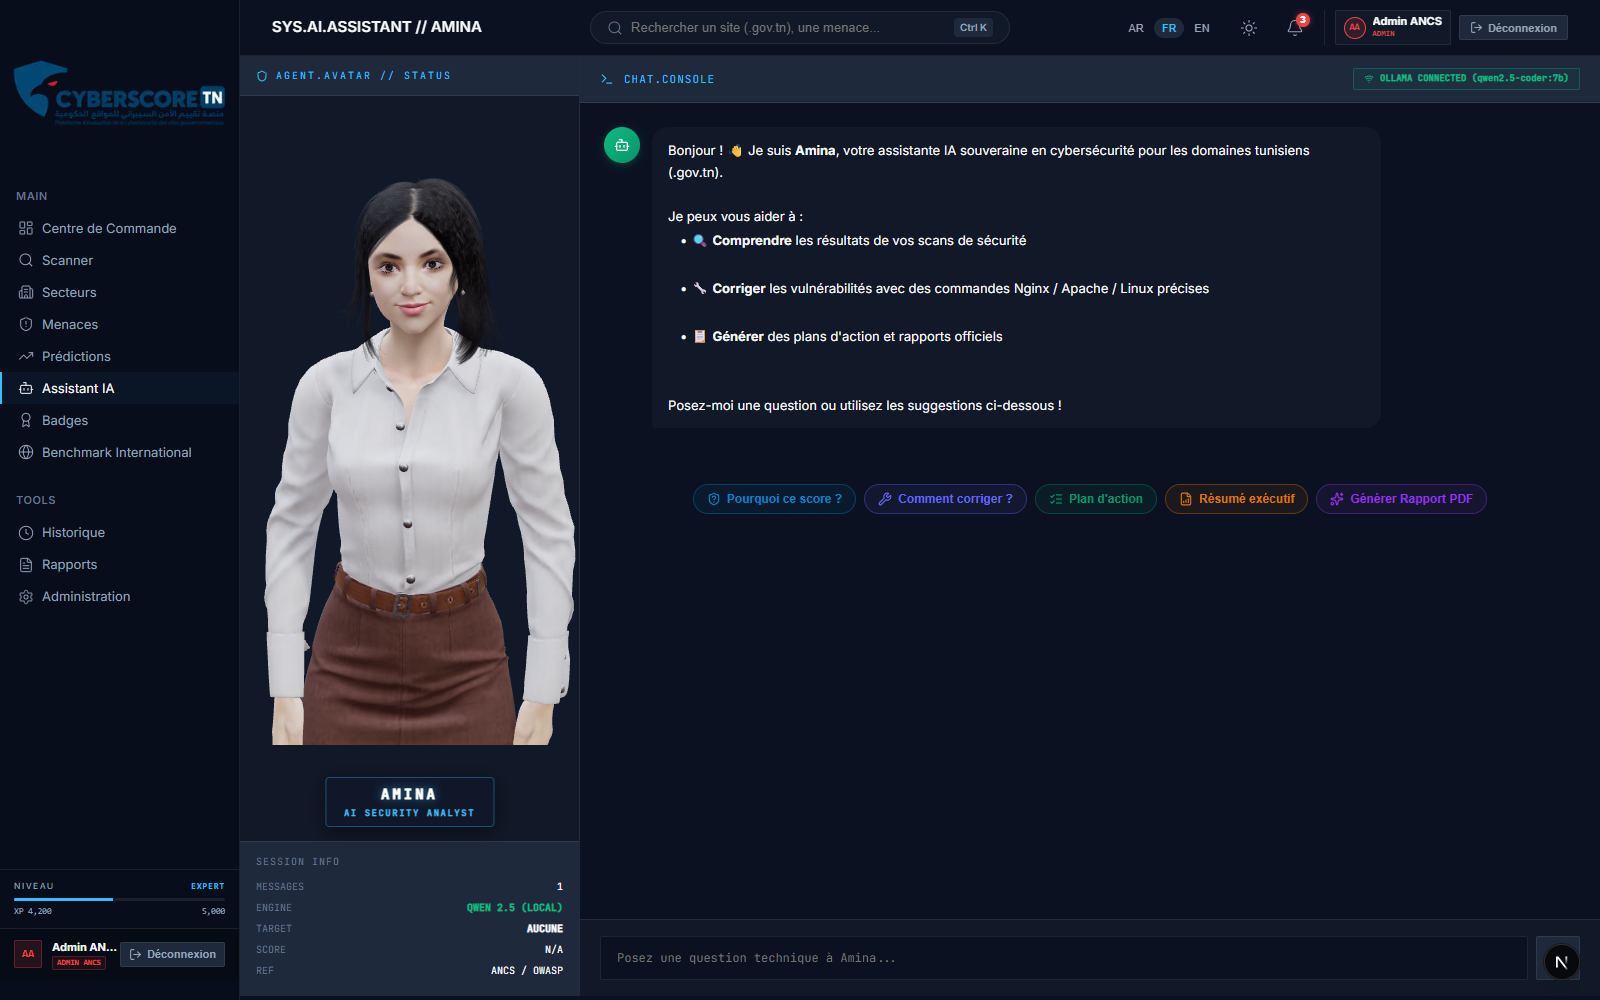
\includegraphics[width=0.70\textwidth]{images/assistant.png}
\caption{Console conversationnelle de l'analyste IA Amina sous Qwen2.5-Coder:7b}
\label{fig:assistant_view}
\end{figure}
